\documentclass{article}

% Packages for setting up page margins
\usepackage[margin=1in]{geometry}

\usepackage{graphicx, setspace, amsmath, mathtools, amssymb, url, float}
\setlength{\parskip}{2mm}
\graphicspath{ {./images/} }

% Title
\title{CS535 Design and Analysis of Algorithms - Assignment 3}
\author{Batkhishig Dulamsurankhor - A20543498}
\date{\today} % Use \date{} for no date

\begin{document}

\maketitle

\begin{enumerate}
  \item To show that $(S,\mathcal{I})$ is a matroid, it must satisfy the following properties.

  \begin{itemize}
    \item First, it has to be a finite and non-empty set. It is trivial and non-empty set $S$ already satisfies it.
    \item Second is a heredity property. Let's say some two columns of $I$ are dependent on each other.
    It is clear that those two columns are also a subset of $I$, in other words $I^\prime\subseteq I$, where $I^\prime$ is set of the two columns.
    So, by heredity property, if $I\in\mathcal{I}$, then $I^\prime\in\mathcal{I}$ must also satifsy, which is a contradiction since we know that $I^\prime$ is not an independent set and $I^\prime\notin\mathcal{I}$.
    Therefore, to satisfy the second property, all columns in $I$ must be linearly independent.
    \item Let's show that exchange property must satisfy with the similar approach to the previous one.
    We have a set $|B|>2$ such that $B\in\mathcal{I}$, but some column $b_i,b_j$ are dependent on each other.
    Let's imagine that we use heredity property and now we have $B^\prime=\{b_i,b_j\}$ which supposed to be $B^\prime\in\mathcal{I}$.
    We know that $|B|>|B^\prime|$ and we can't find an element $b_k$ in $B$ that can make $B^\prime$ part of the independent set.
    In other words, $\forall b_k \in B-B^\prime:B^\prime\cup\{b_k\}\notin\mathcal{I}$, since $B^\prime$ itself contains linearly dependent columns and adding any element can change the fact that it is dependent.
    This contradicts the property that $\exists b_k \in B-B^\prime:B^\prime\cup\{b_k\}\in\mathcal{I}$ and therefore all columns in $B$ must be linearly independent.
  \end{itemize}

  \item
    \begin{enumerate}
      \item Curcuits in the matric matroid are the minimal dependent subsets of columns of matrix $A$.
      Curcuit $C$ is set of columns that are linearly dependent, but every possible proper subset of $C$ is linearly independent.
      \item Suppose $C_1\neq C_2$, then $C_1\subset C_2$ or $C_1$ must be a proper subset of $C_2$.
      We know that both $C_1$ and $C_2$ are dependent sets.
      On the other hand, it is defined that removal of any element in $C$ must result in an independent set.
      So, a proper subset of $C_2$ results in an independent set, which makes $C_1$ an independent set.
      This leads to a contradiction since a set can't be dependent and independent at the same time.
      Thus, if $C_1\subseteq C_2$, then $C_1=C_2$.

      For example, in a graph matroid, minimal dependent subset is a cycle $C=(V,E)$ in the graph.
      In a cycle, the number vertices and the number of edges must be equal, $|V|=|E|$.
      Removing any edge will result in a tree which is an independent set, $|V|=|E|-1$.
      If a cycle $C_1$ is a subset of a cycle $C_2$, the only possible option is that $C_1=C_2$.
      Because removing an edge from a cycle will never result in another cycle, but a tree.
    \end{enumerate}
  \item As mentioned in the problem, jobs do not have start and finish time.
  So the order of execution doesn't matter as long as we choose jobs that maximize the profit.
  The algorithm has an issue and will not always yield the optimal result.

  Our goal is to maximize the profit, so at a glance we have to run jobs that gives the most profit per time frame.
  According to the algorithm, we calculate $p_i/t_i$ for all $i$ jobs and sort them in descending order, which gives us ordered jobs from the most profitable to the least profitable per time frame.
  By greedily choosing from the most profitable job until we can't fit anymore, we can seem to maximize the profit.

  However, the algorithm sometimes fail to achieve the maximum profit since it can look over more profitable combinations by greedily choosing the most profitable job first.
  Let's disprove the correctness of this algorithm with an example.
  Suppose we had machine with time span $T=9$ and $4$ jobs with profit $p=\{10, 21, 8, 14\}$ and required time $t=\{2,7,2,7\}$.

  \begin{itemize}
    \item Calculating $p_i/t_i$ gives the following rates: $r=\{5,3,4,2\}$.
    \item Sorting them by $r$ in descending order gives: $job_1,job_3,job_2,job4$.
    \item Now we greedily choose jobs with above order until we can no longer fit within the timeframe of $T=9$.
    \item We choose $job_1$ and the total profit becomes: $P=p_1=10$, and time left: $T_l=T-t_1=9-2=7$.
    \item Then we choose $job_3$: $P=p_1+p_3=10+8=18$, $T_l=T-t_1-t_3=9-2-2=5$.
    \item Finally, we have only $T_l=5$ left so we can't run anymore jobs since $t_2=7,t_4=7$.
    \item The final answer is $P=18$.
  \end{itemize}

  But, we can clearly see that maximum profit we can make is $P=31$ by choosing $job_1,job_2$.
  They have total required time of $t_1+t_2=9$ which fits in $T=9$.
  So, this greedy algorithm doesn't result in optimal solution.
  Instead, we need to choose other methods, like dynamic programming to solve this problem optimally.
  
  \item
    \begin{enumerate}
      \item This theorem is not correct. Let's look at the following example.

      \begin{figure}[H]
        \centering
        \begin{minipage}{0.4\textwidth}
          \centering
          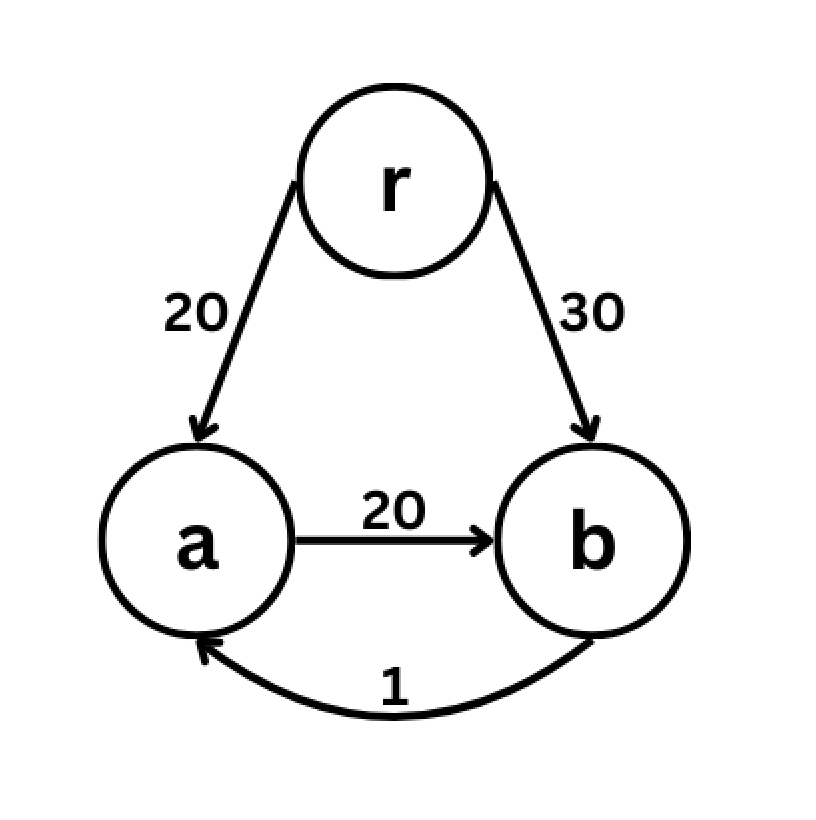
\includegraphics[width=0.7\textwidth]{image1.png}
          \caption{Suppose we had the above graph $(G,w)$. $r$ is the root node.}
        \end{minipage}
        \hspace{1cm}
        \begin{minipage}{0.4\textwidth}
          \centering
          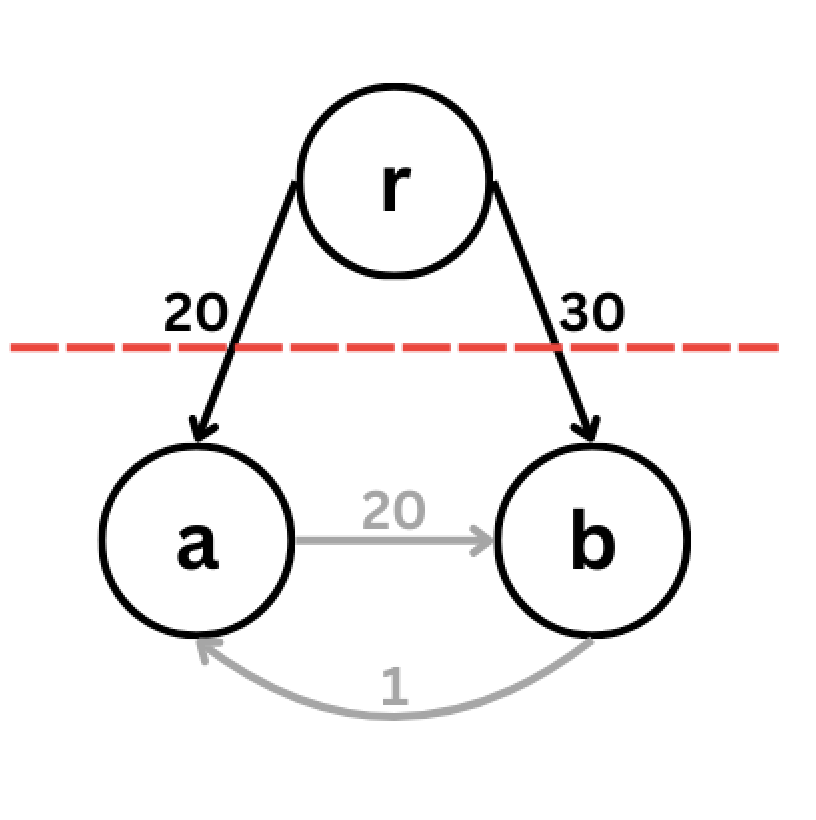
\includegraphics[width=0.7\textwidth]{image2.png}
          \caption{Consider the above cut. $R=\{r\}$ and $V-R=\{a,b\}$. The cut-set $(R,V-R)$ contains edge from $r\rightarrow a$ and $r\rightarrow b$. According to the algorithm, the smalled edge from $R$ to $V-R$ must be a part of minimum weight directed spanning tree, which is an edge $r\rightarrow a$.}
        \end{minipage}
      \end{figure}

      \begin{figure}[H]
        \centering
        \begin{minipage}{0.4\textwidth}
          \centering
          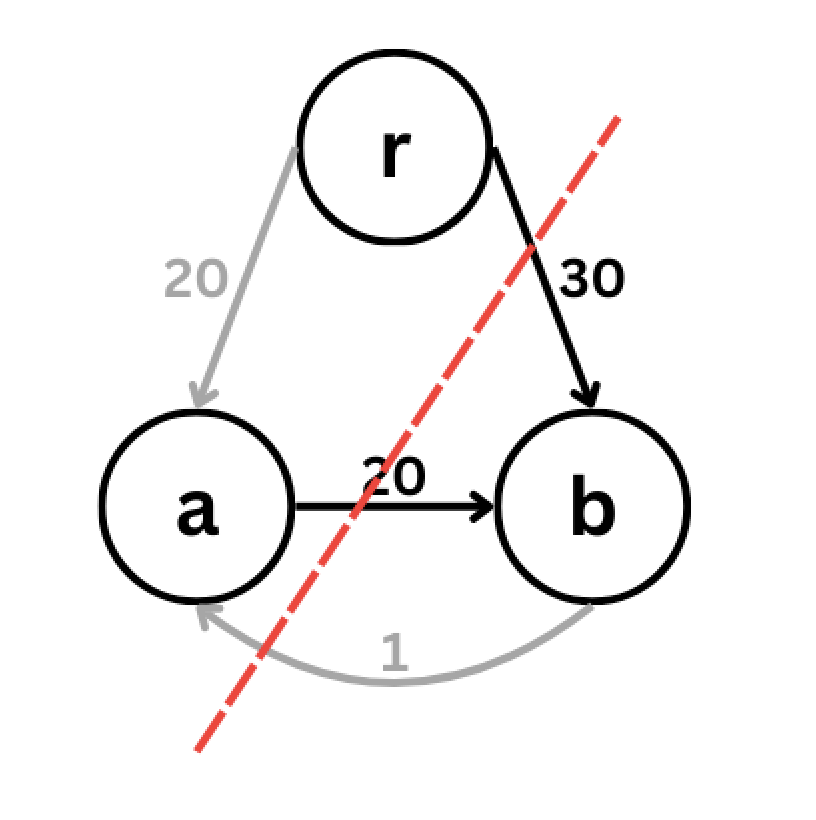
\includegraphics[width=0.7\textwidth]{image3.png}
          \caption{Now $R=\{r,a\}$ and $V-R=\{b\}$. So the the new cut-set becomes $(R,V-R)=\{r\rightarrow b,a\rightarrow b\}$} and the edge $a\rightarrow b$ is part of minimum weight directed spanning tree.
        \end{minipage}
        \hspace{1cm}
        \begin{minipage}{0.4\textwidth}
          \centering
          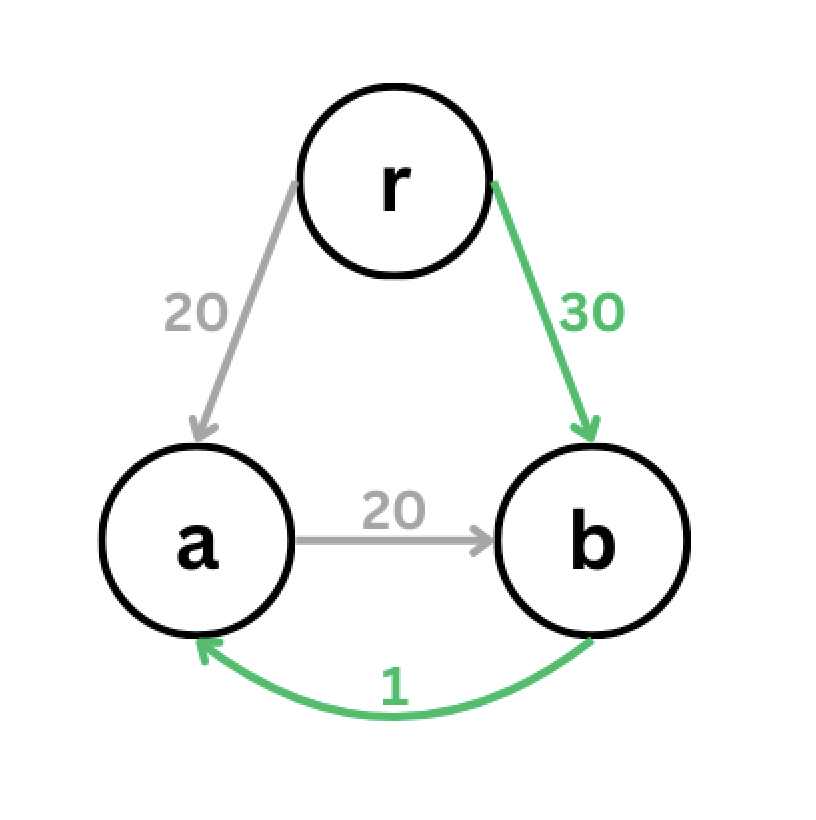
\includegraphics[width=0.7\textwidth]{image4.png}
          \caption{However, minimum weight directed spanning tree consists of edges $(R,V-R)=\{r\rightarrow b,b\rightarrow a\}$ and total weight of $W=30+1=31$. The previous example fails to find the MST in a directed graph.}
        \end{minipage}
      \end{figure}

      Since we can't necessarily have the same weight between edges $a\rightarrow b$ adn $b\rightarrow a$, the tree can take different routes that minimizes the total weight. Therefore, this theorem is false.

      \item hello
    \end{enumerate}
\end{enumerate}

\begin{thebibliography}{9}

\bibitem{master}
master.pdf.

\bibitem{wiki}
Fibonacci sequence, \emph{Wikipedia}, \url{https://en.wikipedia.org/wiki/Fibonacci_sequence#Relation_to_the_golden_ratio}

\end{thebibliography}


\end{document}